\documentclass[aspectratio=169]{beamer}
\usetheme{Singapore}

% add page numbers at the bottom of the slides
\setbeamertemplate{caption}[numbered]
\addtobeamertemplate{navigation symbols}{}{%
    \usebeamerfont{footline}%
    \usebeamercolor[fg]{footline}%
    \hspace{1em}%
    \raisebox{1.4pt}[0pt][0pt]{\insertframenumber/\inserttotalframenumber}
}

% \definecolor{primarycolor}{HTML}{0000FF}

% \makeatletter

% \def\sectioncolor{primarycolor}% color to be applied to section headers

% \setbeamercolor{palette primary}{use=structure,fg=structure.fg}
% \setbeamercolor{palette secondary}{use=structure,fg=structure.fg!75!black}
% \setbeamercolor{palette tertiary}{use=structure,fg=structure.fg!50!black}
% \setbeamercolor{palette quaternary}{fg=black}

% \setbeamercolor{local structure}{fg=primarycolor}
% \setbeamercolor{structure}{fg=primarycolor}
% \setbeamercolor{title}{fg=primarycolor}
% \setbeamercolor{section in head/foot}{fg=black}

% \setbeamercolor{normal text}{fg=black,bg=white}
% \setbeamercolor{block title alerted}{fg=red}
% \setbeamercolor{block title example}{fg=primarycolor}

% \setbeamercolor{footline}{fg=primarycolor!50}
% \setbeamerfont{footline}{series=\bfseries}

% use classic LaTeX font for maths
\usefonttheme[onlymath]{serif}

\usepackage{cmap}
\usepackage[english]{babel}
\usepackage[T1]{fontenc}
\usepackage[utf8]{inputenc}
\usepackage[kerning=true]{microtype}
\usepackage{lmodern}

\usepackage{amsmath}
\usepackage{amsfonts}
\usepackage{amssymb}
\usepackage{amsthm}

\usepackage{mathtools}
\usepackage{tikz}
\usepackage{xcolor}
\usepackage{multirow}
\usetikzlibrary{positioning}

\usepackage[
    backend=biber,
    style=numeric,
]{biblatex}
\usepackage{graphicx}
\usepackage[justification=centering]{caption}
\usepackage{csquotes}

\graphicspath{{../images/}}

\addbibresource{../report/report.bib}
\renewcommand*{\bibfont}{\footnotesize}

\AtBeginSection[]
{
  \begin{frame}
    \frametitle{Plan}
    \tableofcontents[currentsection]
  \end{frame}
}


\theoremstyle{definition}
\newtheorem*{exemple}{Example}

\renewcommand{\leq}{\leqslant}
\renewcommand{\geq}{\geqslant}
\renewcommand{\epsilon}{\varepsilon}
\DeclareMathOperator*{\sign}{sign}
\DeclareMathOperator*{\Clip}{Clip}


\title{\textbf{Adversarial Attacks on Images}}

\author{Pierre-Gabriel Berlureau\and Antoine Groudiev\and Matéo Torrents}

\titlegraphic{
\includegraphics[height=1.6cm]{../images/logo-ens-psl.png}}

\date{\today}

\begin{document}
\frame{\titlepage}

\begin{frame}{Plan}
   \tableofcontents
\end{frame}

\section{Adversarial attacks: taxonomy and goals}
\subsection{Adversarial goals}
\begin{frame}{Definition}
  \begin{itemize}
    \item \textbf{Adversarial image}: an image that has been slightly modified to fool a vision system into making a mistake
    \item \textbf{Usual method}: adding a small perturbation to the image
    \begin{equation*}
      X_{\text{attack}} = X_{\text{original}} + \underbrace{\delta X}_{\text{perturbation}}
    \end{equation*}
  \end{itemize}
  \begin{figure}
    \centering
    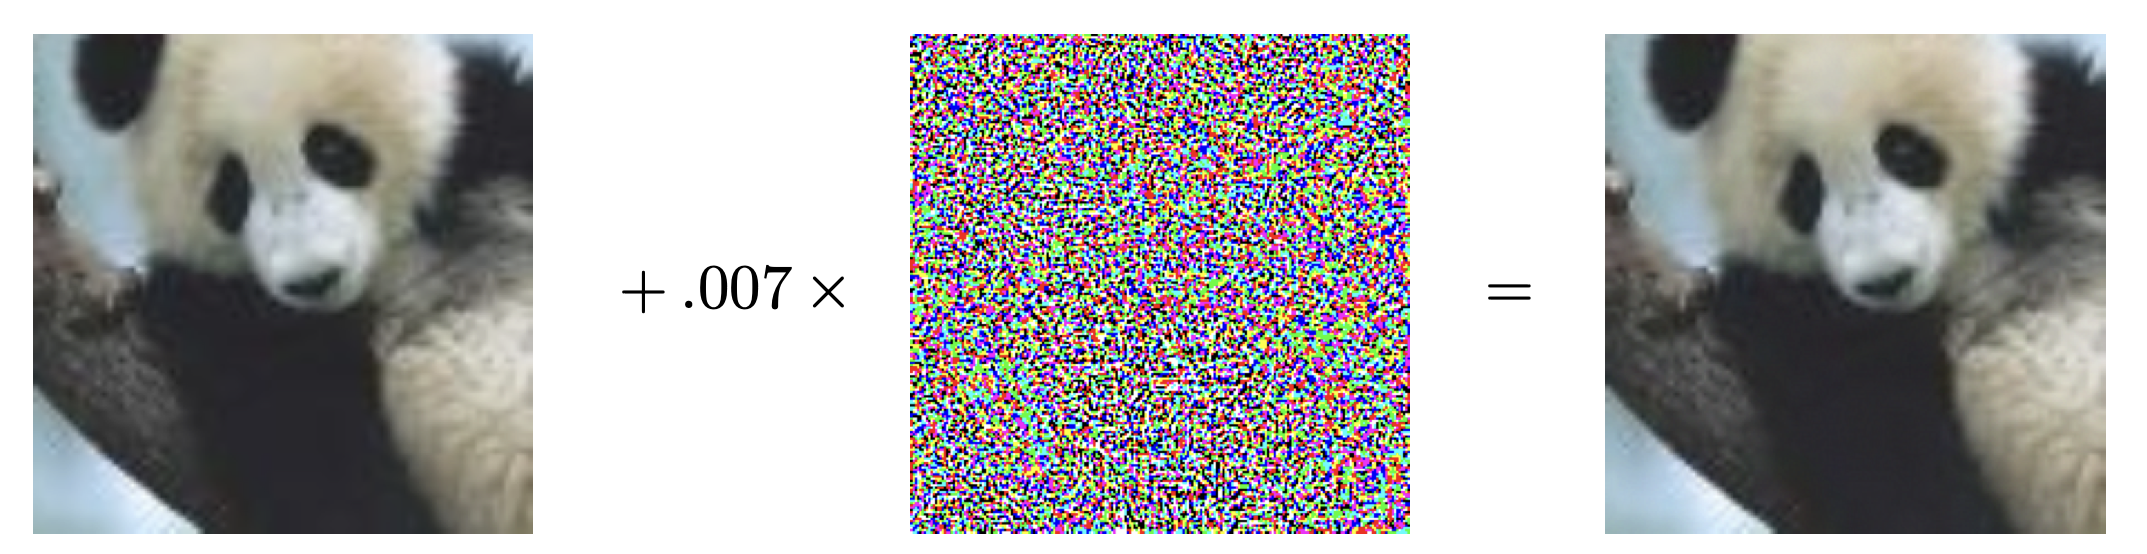
\includegraphics[width=0.8\textwidth]{panda.png}
  \end{figure}
\end{frame}
\begin{frame}{Adversarial goals}
\textbf{Goals of the attack}:
\begin{itemize}
  \item \textbf{Confidence reduction}: reduce the confidence of the model in its prediction
  \item \textbf{Misclassification}: make the model predict a different class, "evasion"
  \item \textbf{Source/target misclassification}: make the model predict a specific class
  \item For binary systems, \textbf{non-detection} (i.e. "invisibility" to the model)
\end{itemize}
\end{frame}
\subsection{Adversarial capabilities}
\begin{frame}{Adversarial capabilities}{Training v. testing phase approaches}
  \begin{figure}
    \centering
    \begin{minipage}{0.4\textwidth}
      \centering\textbf{Training phase approach}
      \begin{itemize}
        \item Corrupt the training phase of the model by altering the images
        \item Automatically misclassify \emph{legitimate} images
      \end{itemize}
    \end{minipage}
    \hspace{0.1\textwidth}
    \begin{minipage}{0.4\textwidth}
      \centering\textbf{Testing phase approach}
      \begin{itemize}
        \item The model is already trained on clean images
        \item Misclassify \emph{adversarial} images
      \end{itemize}
    \end{minipage}
  \end{figure}
\end{frame}

\begin{frame}{Adversarial capabilities}{White-box v. black-box approaches}
  \begin{figure}
    \centering
    \begin{minipage}{0.4\textwidth}
      \centering\textbf{White-box approach}
      \begin{itemize}
        \item Full access to a copy of the model
        \item Knowledge of the model's architecture and parameters
        \item Query the model
        \item Differentiate the model
      \end{itemize}
    \end{minipage}
    \hspace{0.1\textwidth}
    \begin{minipage}{0.4\textwidth}
      \centering\textbf{Black-box approach}
      \begin{itemize}
        \item Access to the model as an oracle only
        \item Sometimes, access to pre-queried tuples $(x,y)$
        \item Common approach: train a surrogate model using the queried examples
      \end{itemize}
    \end{minipage}
  \end{figure}
\end{frame}

\subsection{Real-world examples}
\begin{frame}{Real-world examples}
  \begin{itemize}
    \item Biometric identification systems
    \item Attack autonomous vehicles by modifying road signs
    \item Modify license plates to evade detection/identification
  \end{itemize}
\end{frame}

\section{Attacks algorithms}
\subsection{Fast Gradient Sign Method (FGSM)}
\begin{frame}{Fast Gradient Sign Method (FGSM)}{Classical setup}
  We want to reduce the confidence of the model in its prediction. For an image $X$ of initial class $y_{\text{true}}$:
  \begin{equation*}
    X_* = X + \epsilon\sign\left(\nabla_x J(X, y_{\text{true}})\right)
  \end{equation*}
  with $J$ the loss function and $\epsilon$ the amplitude of the changes.
  % If we have white-box access to the model, $\nabla_x J$ is easy to compute.
  \begin{figure}
    \centering
    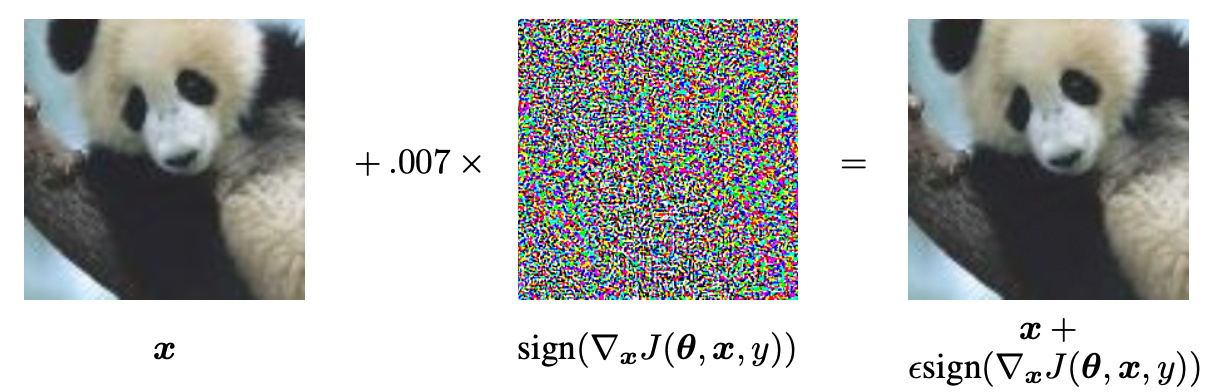
\includegraphics[width=0.7\textwidth]{panda-fgsm.png}
  \end{figure}
\end{frame}

\begin{frame}{Fast Gradient Sign Method (FGSM)}{Source/target misclassification}
  We want to misclassify the image as a specific class $y_{\text{target}}$:
  \begin{equation*}
    X_* = X - \epsilon\sign\left(\nabla_x J(X, y_{\text{target}})\right)
  \end{equation*}
  We want to maximize the confidence for $y_{\text{target}}$, therefore minimizing the loss $J$, hence the minus sign.
\end{frame}

\begin{frame}{Fast Gradient Sign Method (FGSM)}{Iterating}
  Iterating over multiple steps of gradient evaluation:
  \begin{equation*}
    \begin{cases*}
        X_*^0 \quad= X\\
        X^{n+1}_* = \Clip\left(X^n_*-\alpha\sign\left(\nabla_x J(X^n_*, y_{\text{true}})\right)\right)
    \end{cases*}
  \end{equation*}
  Such a method is usually stronger than FGSM as it results in smaller and more precise steps instead of one big step in the original gradient direction.
\end{frame}

\begin{frame}{Fast Gradient Sign Method (FGSM)}{Results}
  \begin{figure}
    \centering
    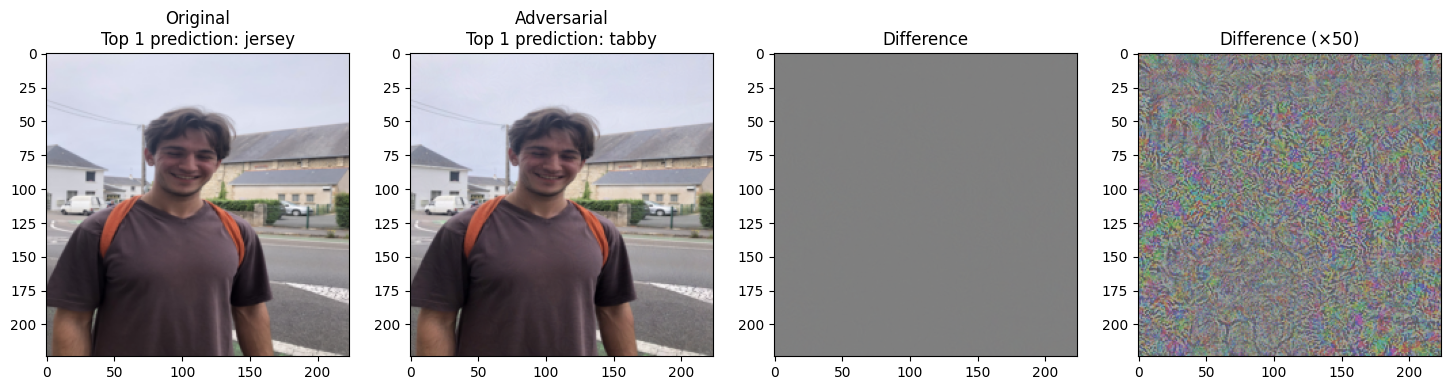
\includegraphics[width=\textwidth]{fgsm-tabby.png}
    \caption{Iteration of FGSM to misclassify an image as \texttt{tabby}\\(model: \texttt{ResNet-18}; iterations: 6; $\alpha=0.001$)}
  \end{figure}
\end{frame}

\subsection{Facial accessories}
\begin{frame}{Facial accessories}
  \begin{figure}
    \centering
    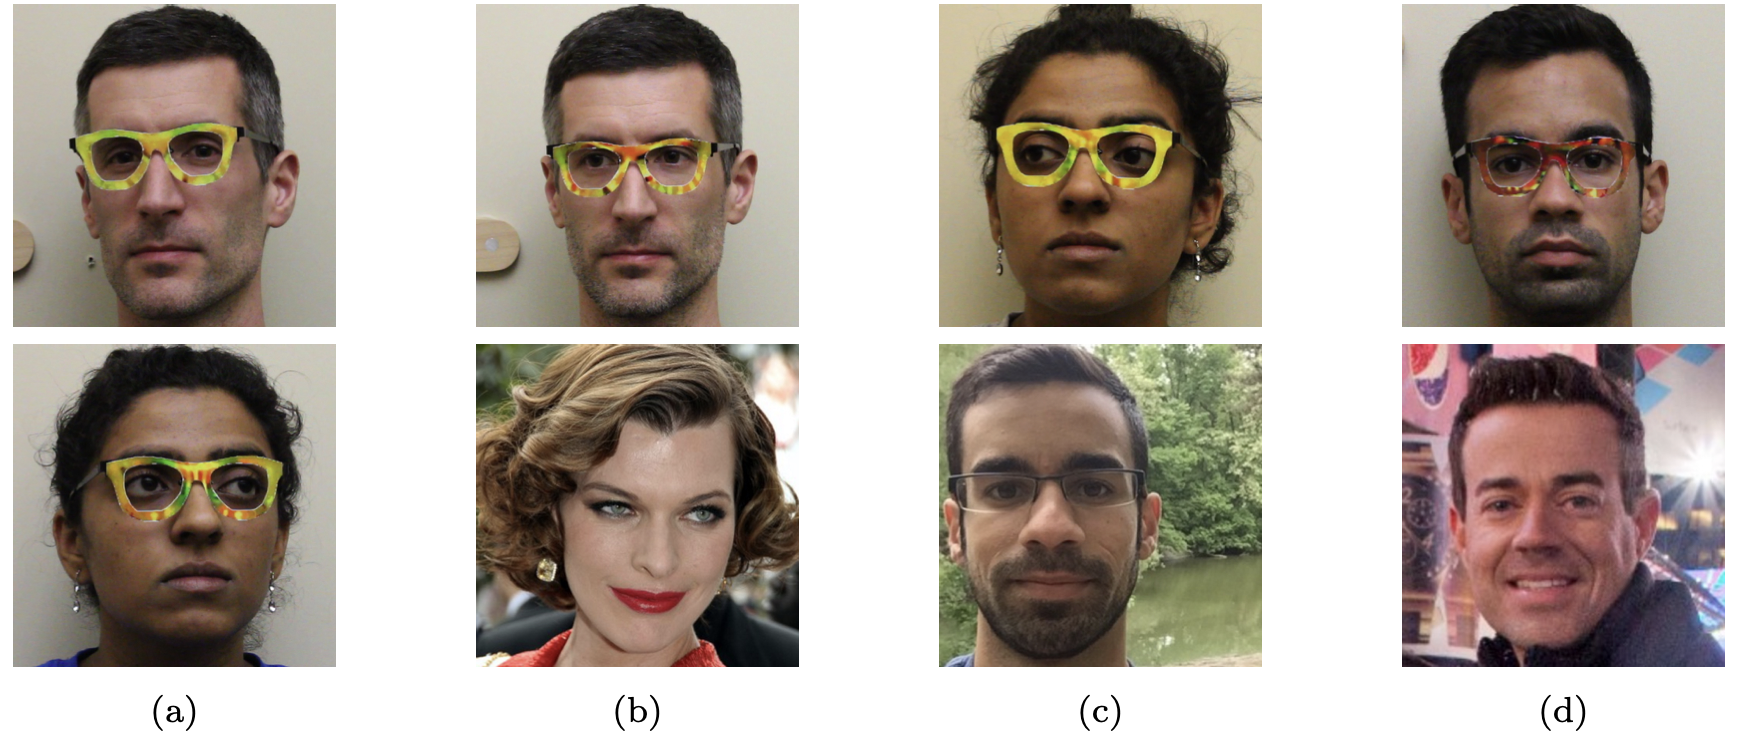
\includegraphics[width=0.8\textwidth]{facial-accessories.png}
    \caption{Facial accessories used to fool facial recognition systems\\ (source: \cite{sharif2016accessorize})}
  \end{figure}
\end{frame}

\section{Defense mechanisms}
\subsection{Adversarial training}
\begin{frame}{Adversarial training}
  \begin{itemize}
    \item \textbf{Idea}: teach the model to be robust to adversarial images by showing it adversarial examples during training
    \item Training with a modified loss function:
    \begin{equation*}
      \tilde{J}_\theta(x, y) = \alpha J_\theta(x, y) + (1-\alpha)J_\theta\Bigl(\underbrace{x+\epsilon\sign\left(\nabla_x J_\theta(x, y)\right)}_{\text{FGSM attack}}\Bigr)
    \end{equation*}
    where $\alpha$ is typically set to $0.5$
  \end{itemize}
\end{frame}

\subsection{\texttt{NULL} labeling}
\begin{frame}{\texttt{NULL} labeling}
  \begin{itemize}
    \item \textbf{Idea}: allow the model to reject adversarial examples
    \item \textbf{Procedure}:
    \begin{enumerate}
      \item Train a classifier on clean images
      \item Introduce a new \texttt{NULL} label
      \item Compute adversarial examples using the clean dataset with different amplitudes, and assign to each a \texttt{NULL} probability depending on this amplitude
      \item Continue to train the classifier on both the clean and adversarial images
    \end{enumerate}
  \end{itemize}
\end{frame}

\subsection{Results comparison}
\begin{frame}{Results comparison}
  \begin{figure}
    \centering
    \renewcommand{\arraystretch}{1.2}
    \begin{tabular}{|c|c|p{3.7cm}||c|c|}
      \hline
      Dataset & Model & \centering Defense & Real data acc. & Adversarial data acc.\\
      \hline\hline
      \multirow{3}{*}{\texttt{MNIST}} & \multirow{3}{*}{CNN} & None & 99\% & 70\%\\\cline{3-5}
      && Adversarial training & 99\% & 95\%\\\cline{3-5}
      && \texttt{NULL} labeling & 99\% & 99\%\\\hline
    \end{tabular}
  \end{figure}
\end{frame}

\section{Conclusion}
\begin{frame}{Conclusion}
  \begin{itemize}
    \item Simple yet effective methods allow attackers to fool highly accurate computer vision systems
    \item Defense mechanisms are still not fully efficient
    \item The threat of adversarial images for computer vision systems is a major issue
    \item Open-source models are particularly vulnerable
  \end{itemize}
\end{frame}


\begin{frame}{References}
    \nocite{*}
    \printbibliography
\end{frame}

\end{document}